\documentclass[a4paper,12pt]{article}
%\documentclass[12pt, landscape, twocolumn]{article}

% Custom margins
%\usepackage[a4paper, inner=1.7cm, outer=2.7cm, top=2cm,  bottom=2cm, bindingoffset=1.2cm]{geometry}

\usepackage{blindtext}
\usepackage{lipsum}

\usepackage{graphicx}  %for figures
% Math
\usepackage{amsthm,amssymb}
\usepackage{amsmath}
\usepackage{amsfonts}
\usepackage{amssymb}
\usepackage{physics}

% Problem environment
\newenvironment{problem}[2][Problem]{\begin{trivlist}
\item[\hskip \labelsep {\bfseries #1}\hskip \labelsep {\bfseries #2.}]}{\end{trivlist}}


\usepackage{xspace}
\newcommand{\A}{\ensuremath{\mathcal{A}}\xspace}
\newcommand{\B}{\ensuremath{\mathcal{B}}\xspace}
\newcommand\pa[1]{\ensuremath{\left(#1\right)}}

% Example: download a usepackage 
%\usepackage{CJK}

\usepackage[super]{nth}
% the package for 1st, 2nd etc

\usepackage{setspace}
\doublespacing
% change the line spacing!

\begin{document}


\title{Assignment 3}
\author{Siwen Zhang \\
ECON 833: Computational Methods for Economists}
\date{Fall 2021}
\maketitle


\begin{problem}{1. SPACs Deal Timelines}
	The Figure \ref{fig:SPACtl} below lists 180 closed deals ranging from January, 2015 and June, 2021. Each red line measures the length of a SPAC deal from the beginning date as the IPO date to the end date as the deal closed date. Longer the red line is, more time the deal takes to close. We observe a boom of SPAC deals since 2020, so the blue dashed line separates deal into two parts. The left part includes deals which went public and actively looked for a deal before January \nth{1}, 2020 while the right part contains deals after. Generally, deals before the boom year have relatively longer length compared to more recent deals.\par
	In terms of this figure, I am considering to do more, such as, adding more info to fill the blank area, using different colors to distinguish groups based on different criteria and so on.
\end{problem}


\begin{problem}{2. Daily Average Media Attention and Trading Volume}
	The Figure \ref{fig:mediaAtt} scatters  average daily Twitter and news publication counts, in blue and red respectively, on a SPAC which are sorted on the log average daily trading volume. It shows a clear positive relationship between social media attention and daily trading volume. Moreover, it indicates the variance of Twitter attention is large in the sample compared to that of news attention. The blue dotted line is the average daily Twitter count while the red one is the average news count in the sample.\par
	To improve this figure further, I am thinking to fill up the blank and provide more information on the distribution of both two averages (even two fitted lines). Moreover, it would be interesting to note these outliers' names as readers may find them familiar.
\end{problem}



\begin{problem}{3. SPACs Deal Timelines}
	The Figure \ref{fig:subs} plot the subsamples of series issuers (in blue) and non-series issuers (in red). As series issuers always share the same name with a number added, investors may find them more familiar. Hence, they are able to attract more attention on Twitter - daily average Twitter count for each firm (the second row figures). This investor attention may lead to an easier or better deal with a lower redemption rate (the first row figures), that is, more investors are willing to hold the stock rather than redeeming them for cash.\par
	For a better figure, first I want to add a title for the first row figures and another one for the second row two. Also, adjusting the color and style is useful, and more information about series issuers, such as how many companies with this issuer in total, will be interesting.
\end{problem}


\begin{figure}[h]
	\centering
	\caption{Deal Length for 180 Closed SPAC Deals}
	\label{fig:SPACtl}
	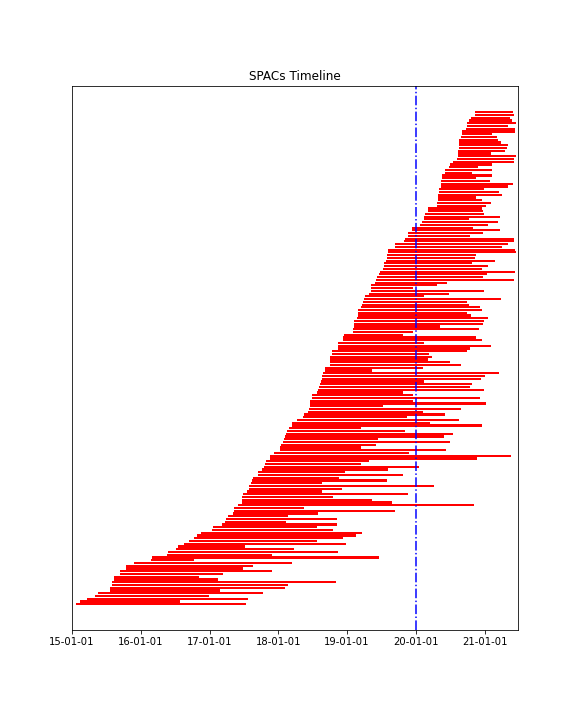
\includegraphics[scale=0.9]{SPACs_tl.png}
\end{figure}

\begin{figure}[h]
	\centering
	\caption{Daily Average Media Attention and Trading Volume}
	\label{fig:mediaAtt}
	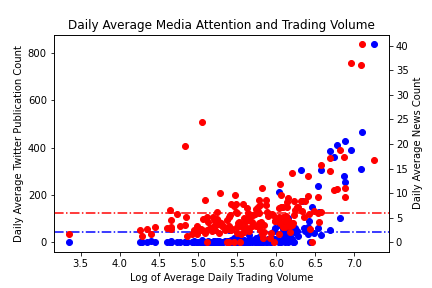
\includegraphics[scale=0.9]{daily_avg_media.png}
\end{figure}

\begin{figure}[h]
	\centering
	\caption{Series Issuers versus Non-series Issuers}
	\label{fig:subs}
	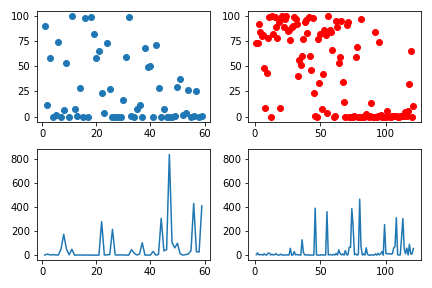
\includegraphics[scale=0.9]{subsample.png}
\end{figure}

\end{document}
